% ---------------------------------------------------------------------------- %
\begin{figure}[htbp]
	\centering
	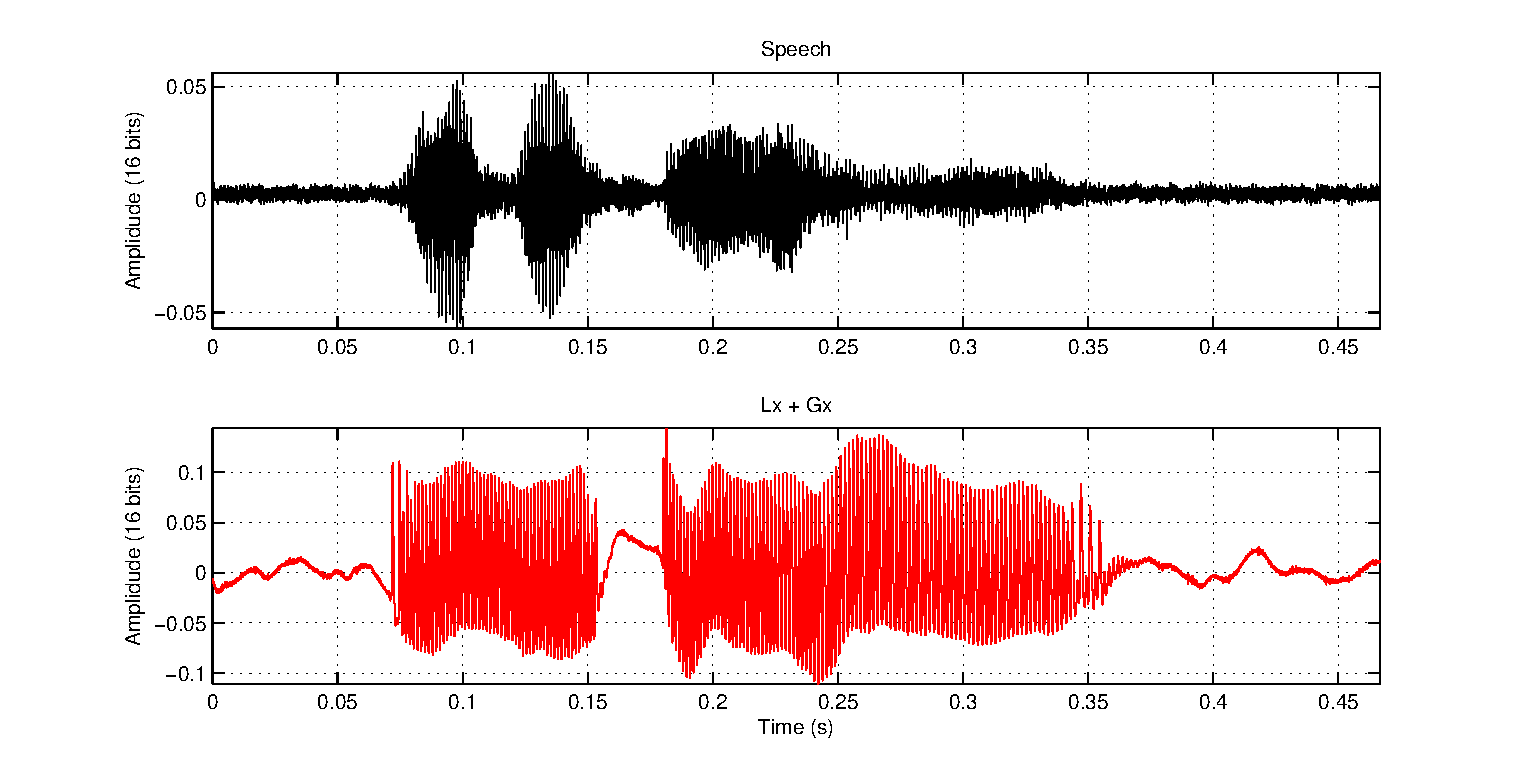
\epsfig{file=include/linguometer/images/lg_example.eps, width=1.00\textwidth}
	\caption[Laryngograph signals]{\textbf{Laryngograph signals}: speech signal 
	(on the top) and EGG signal (on the bottom) acquired with the Laryngograph
	Microprocessor by Laryngograph Ltd.
	The signals were acquired from a 27 years old female subject saying the
	Italian word /lavatoio/ (/sink/ in English).
	The sampling frequency is 16 kHz for both signals.
	The low-frequency component of the EGG signal (Gx signal) is clearly visible 
	before the onset and after the utterance. 
	}
	\label{fig:linguometer:lg:example}
\end{figure}
% ---------------------------------------------------------------------------- %
